\documentclass{beamer}

\usefonttheme{professionalfonts} % using non standard fonts for beamer
\usefonttheme{serif} % default family is serif

\usepackage{hyperref}

%\usepackage{minted}

\usepackage{animate}

\usepackage{graphicx}

\def\Put(#1,#2)#3{\leavevmode\makebox(0,0){\put(#1,#2){#3}}}

\usepackage{color}

\usepackage{tikz}

\usepackage{amssymb}

\usepackage{enumerate}


\newcommand\blfootnote[1]{%

  \begingroup

  \renewcommand\thefootnote{}\footnote{#1}%

  \addtocounter{footnote}{-1}%

  \endgroup

}

\makeatletter

%%%%%%%%%%%%%%%%%%%%%%%%%%%%%% Textclass specific LaTeX commands.

 % this default might be overridden by plain title style

 \newcommand\makebeamertitle{\frame{\maketitle}}%

 % (ERT) argument for the TOC

 \AtBeginDocument{%

   \let\origtableofcontents=\tableofcontents

   \def\tableofcontents{\@ifnextchar[{\origtableofcontents}{\gobbletableofcontents}}

   \def\gobbletableofcontents#1{\origtableofcontents}

 }

%%%%%%%%%%%%%%%%%%%%%%%%%%%%%% User specified LaTeX commands.

\usetheme{Malmoe}

% or ...

\useoutertheme{infolines}

\addtobeamertemplate{headline}{}{\vskip2pt}



\setbeamercovered{transparent}

% or whatever (possibly just delete it)

\makeatother

\begin{document}
\title[DCEL report]{RIDIR Report}
\author[AC]{Andres Calderon}
\institute[Fall'19]{University of California, Riverside}
\makebeamertitle
\newif\iflattersubsect

\AtBeginSection[] {
    \begin{frame}<beamer>
    \frametitle{Outline} 
    \tableofcontents[currentsection]  
    \end{frame}
    \lattersubsectfalse
}

\AtBeginSubsection[] {
    \begin{frame}<beamer>
    \frametitle{Outline} 
    \tableofcontents[currentsubsection]  
    \end{frame}
}

\begin{frame}{Working on Edge Partitioner}
{Fixing issue with empty cells}
    \begin{itemize}
        \item Exploring the option to query the quadtree but it has important drawbacks:
        \begin{itemize}
            \item Edge information at each node is removed after partitioning, so it is not broadcasted to the other nodes.
            \item Even if we have access to edge information, it stores just a sample of the full dataset.
        \end{itemize}
        \item Fixing the issue by mantaining a list of cells covered by a single polygon.
        \begin{itemize}
            \item Pros: Quite simple. The overcost is not significant at this stage.
            \item Cons: It requires partitioning the polygon layer using the edge grid.
        \end{itemize}
    \end{itemize}
\end{frame}

\begin{frame}{Working on Edge Partitioner}
{Fixing issue with empty cells}
    \centering 
    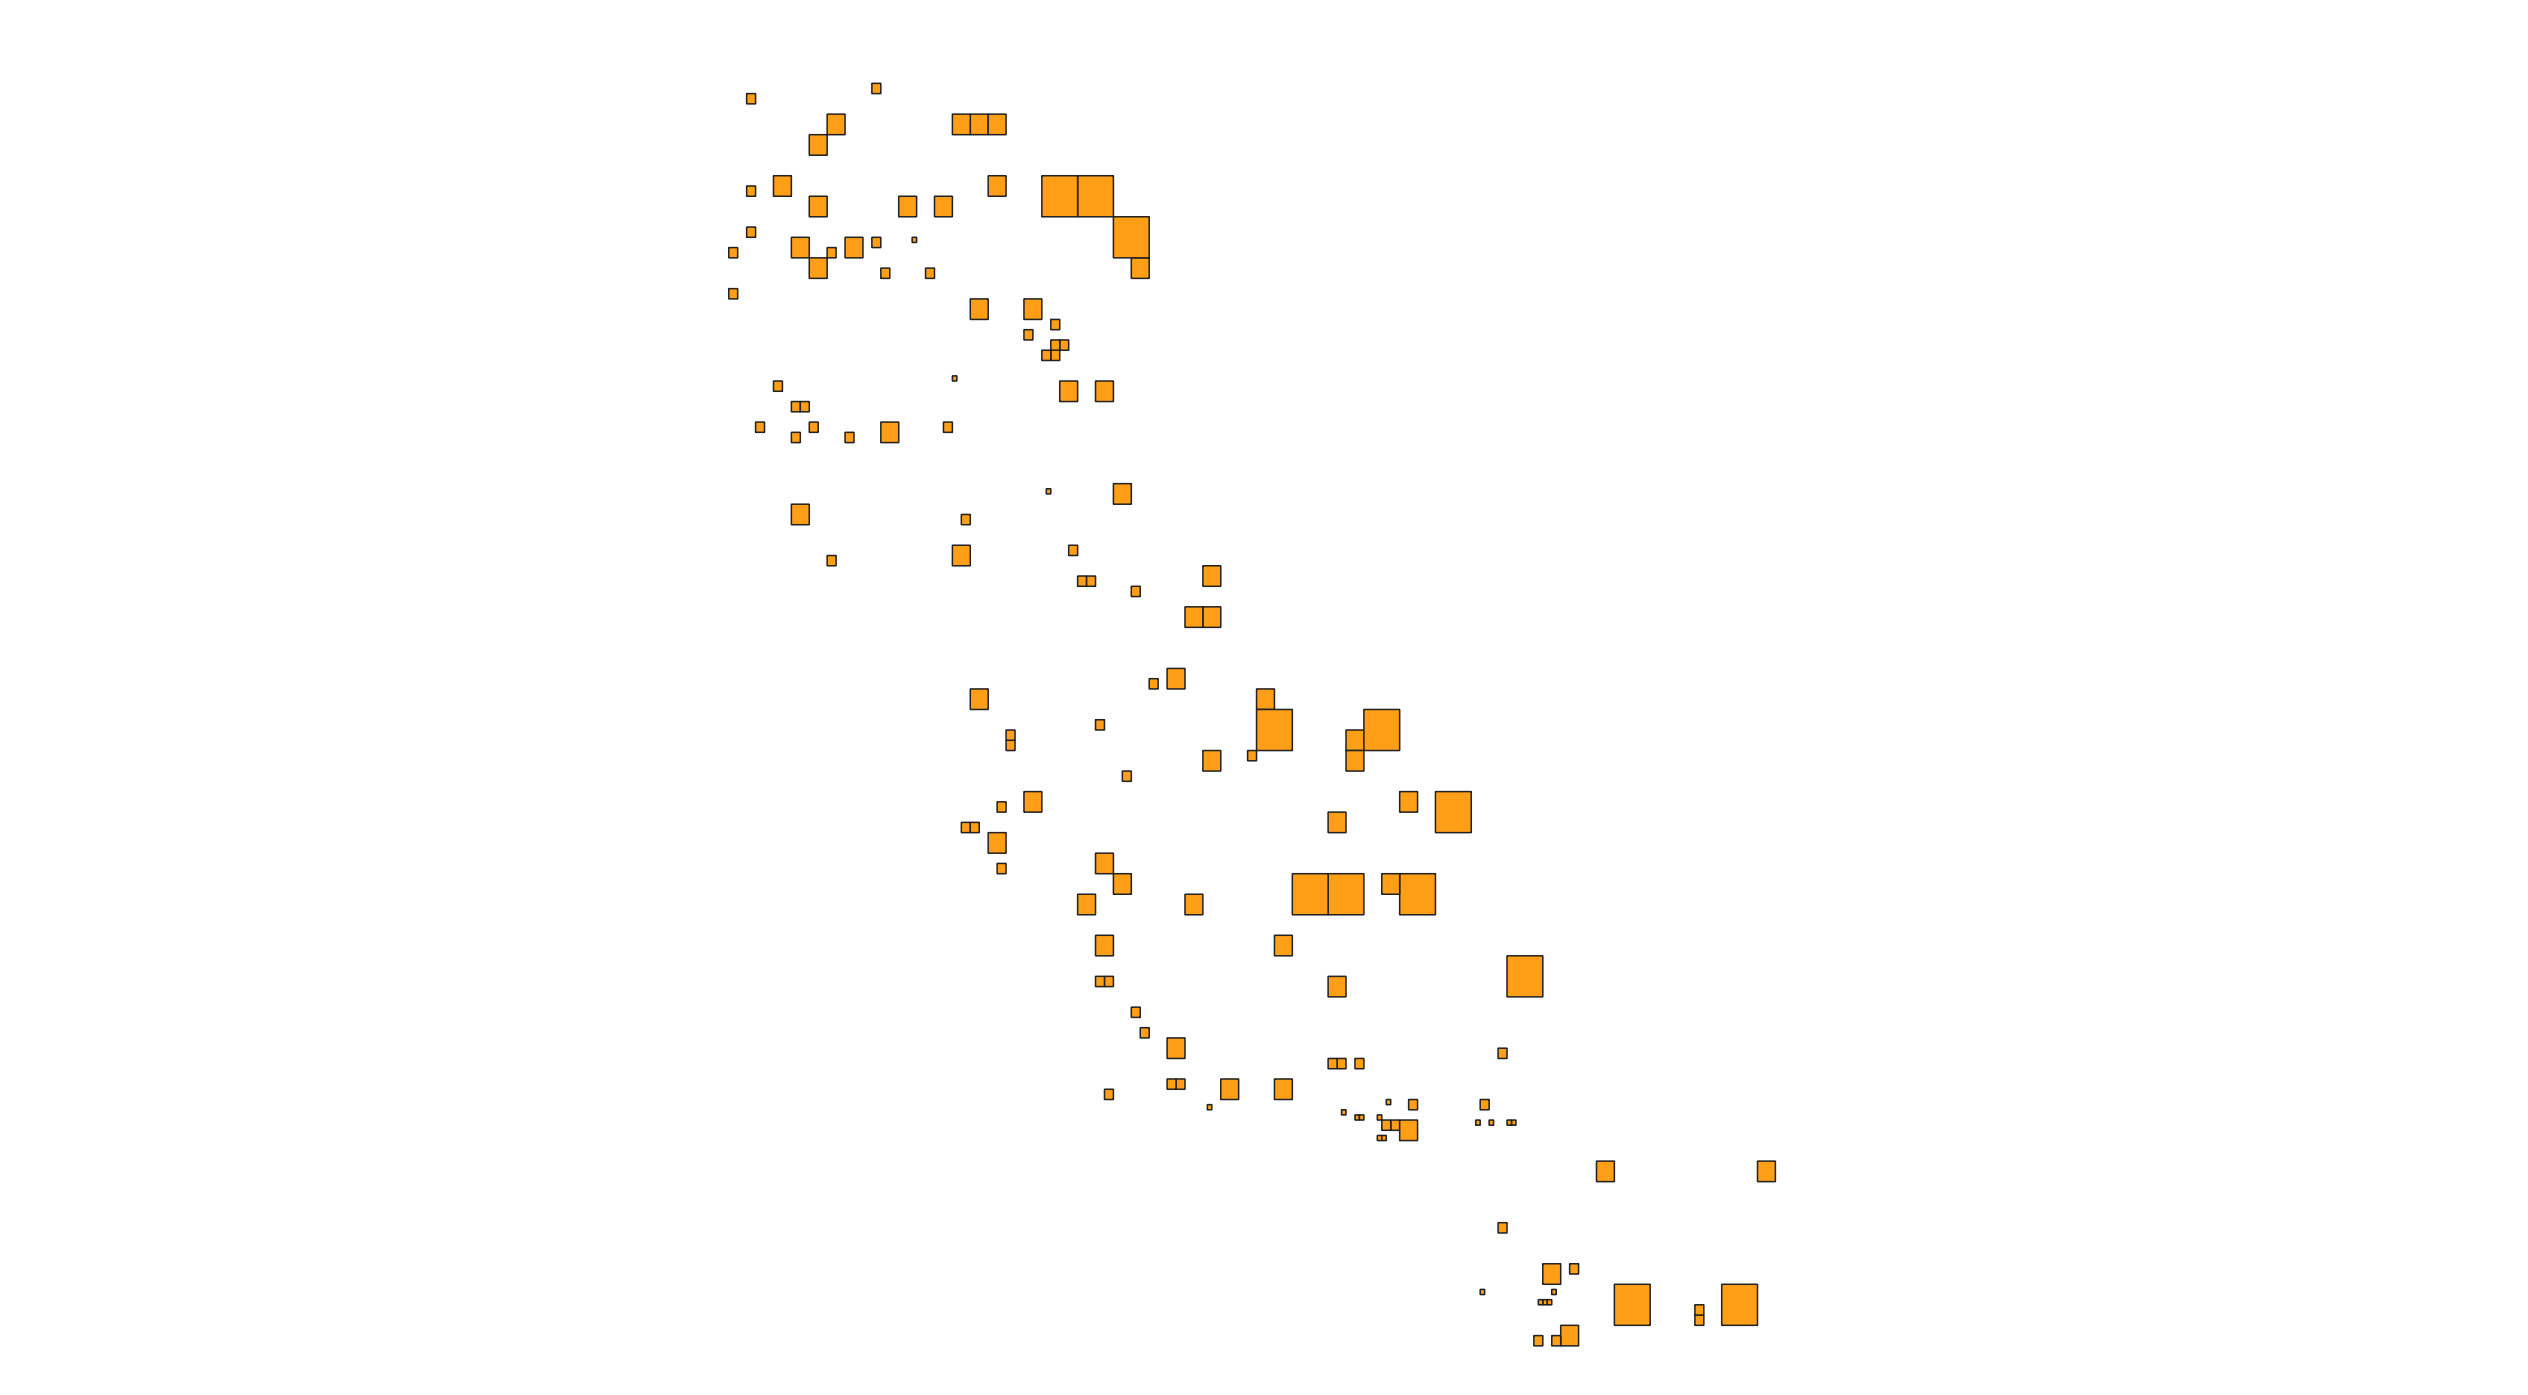
\includegraphics[width=\linewidth]{figures/CA_emptyCells}     
\end{frame}

\begin{frame}{Working on Edge Partitioner}
{Fixing issue with empty cells}
    \centering 
    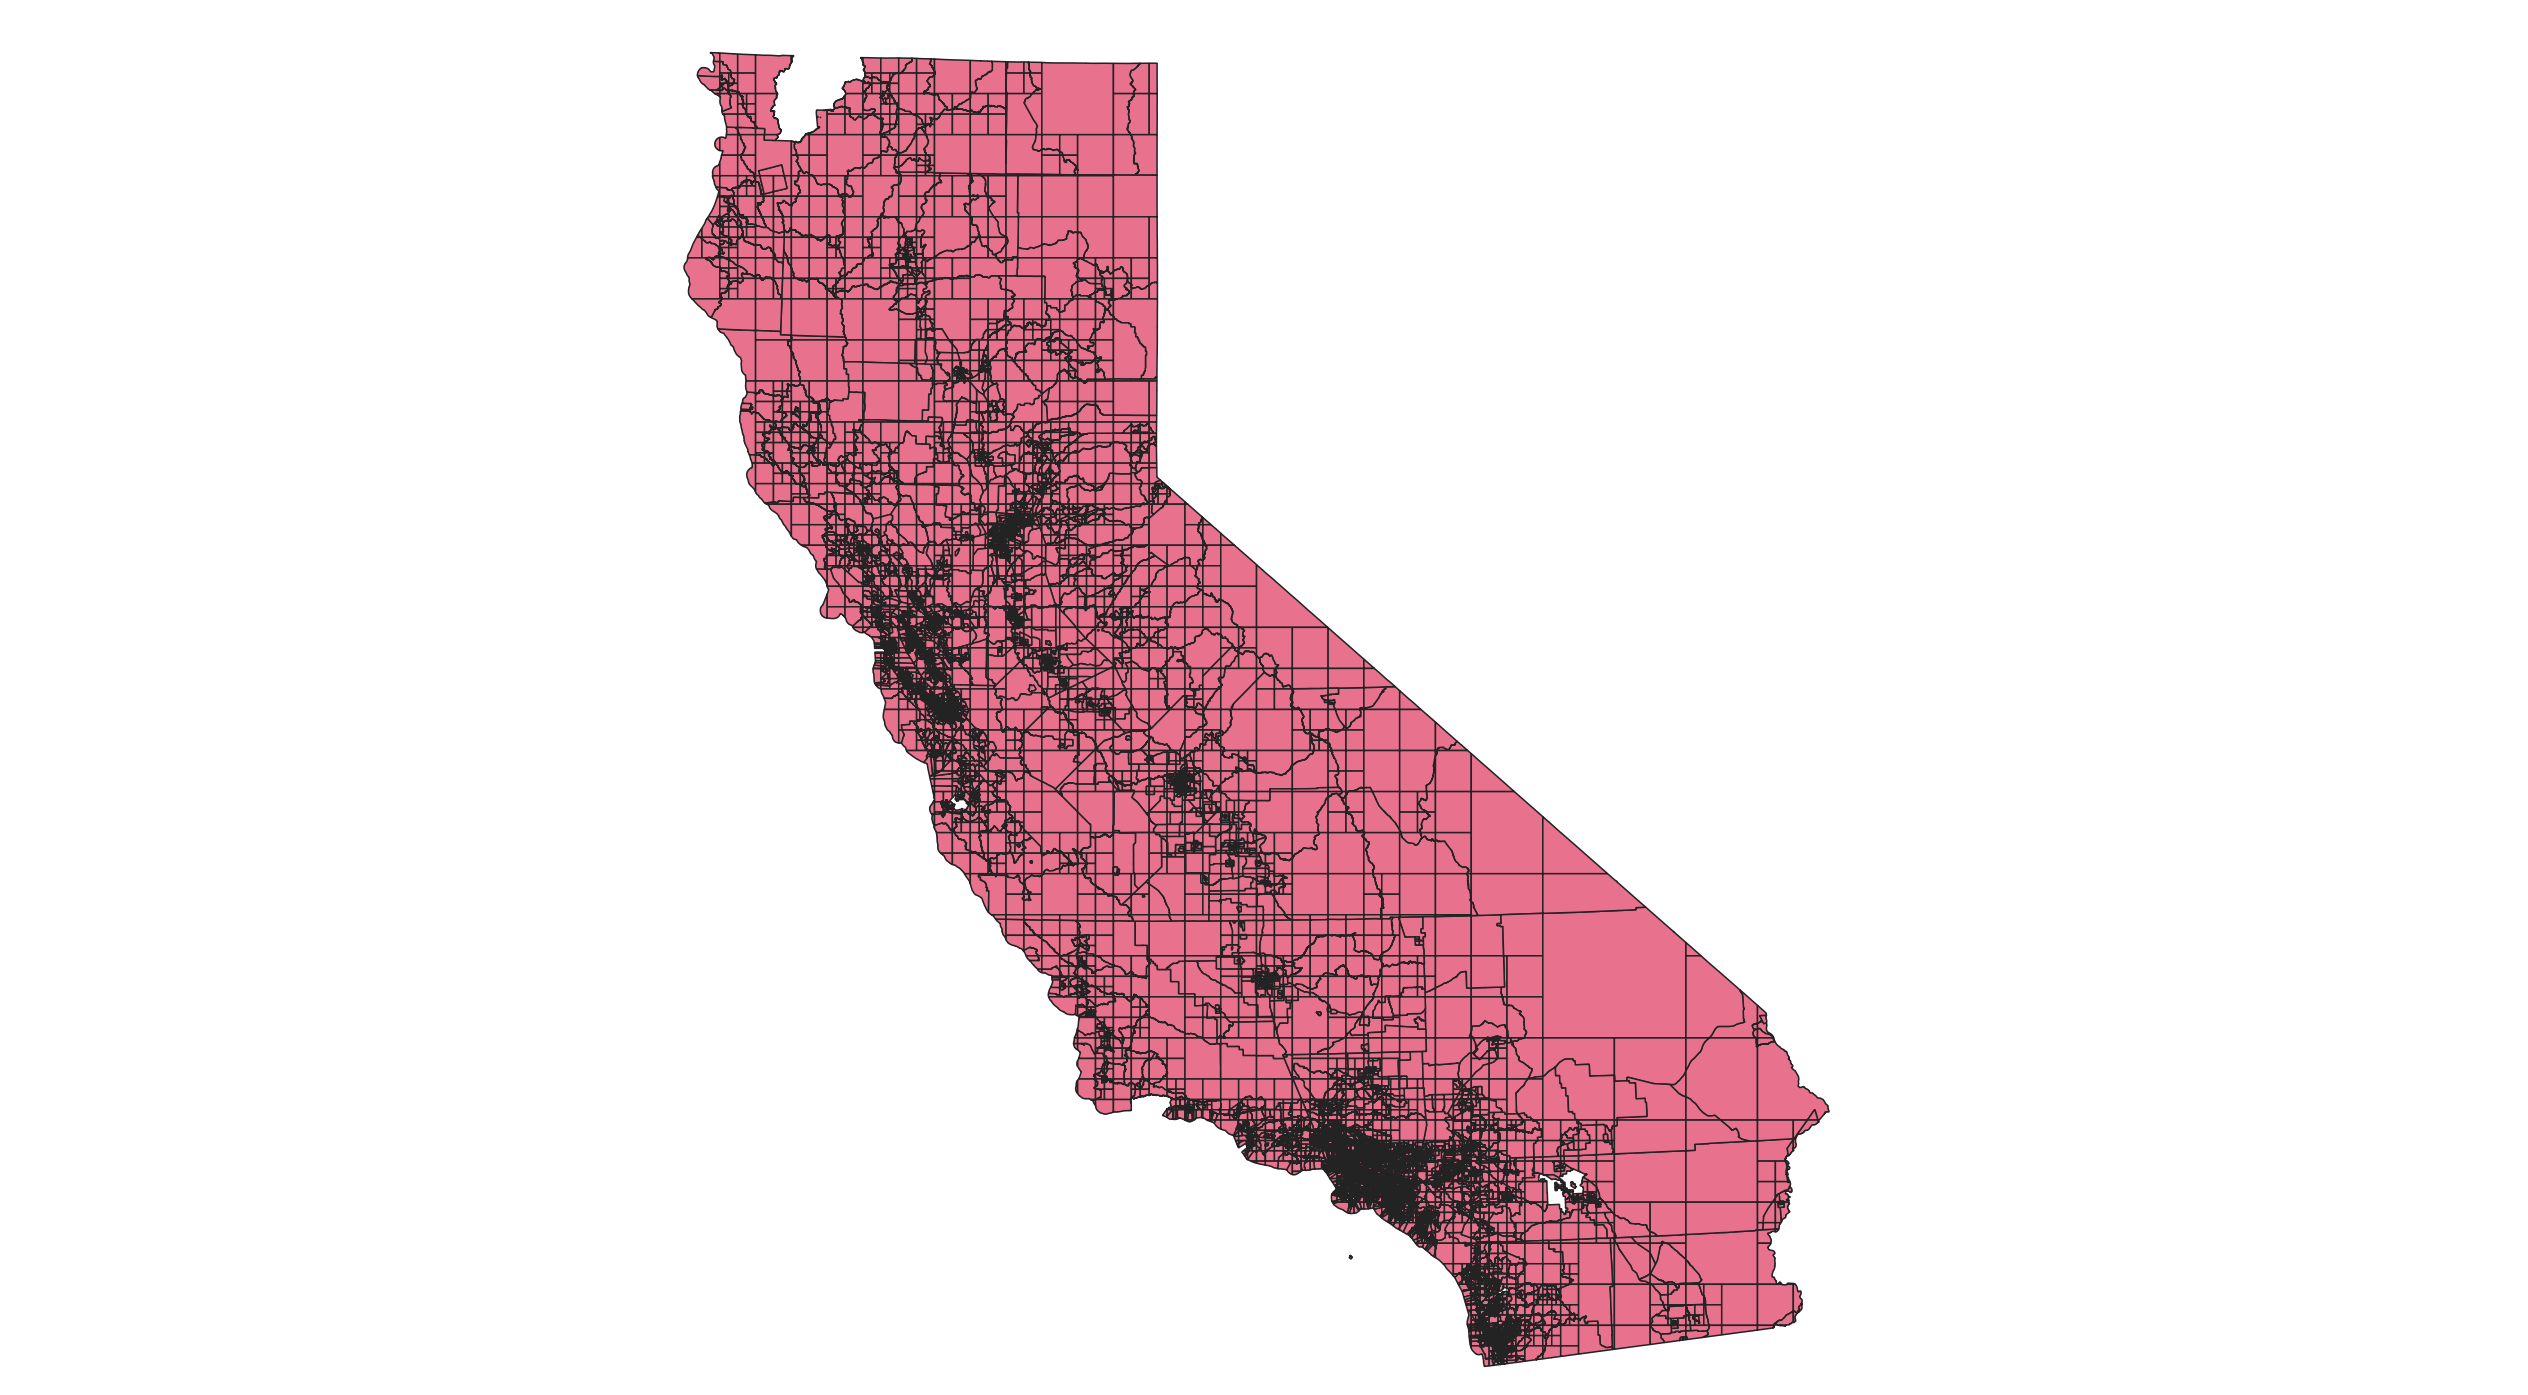
\includegraphics[width=\linewidth]{figures/CA_faces}     
\end{frame}

\begin{frame}{What is next?}
    \begin{itemize}
        \item Integrate the new implementation into the merged DCEL code.
        \item Run experiments in CA\_district datasets.
        \item Explore new dataset.
    \end{itemize}
\end{frame}

\end{document}
